%\begin{figure}
%\captionsetup[subfigure]{labelformat=empty}
%\begin{center}
%	\begin{subfigure}[h]{1.2in}
%		\centering
%		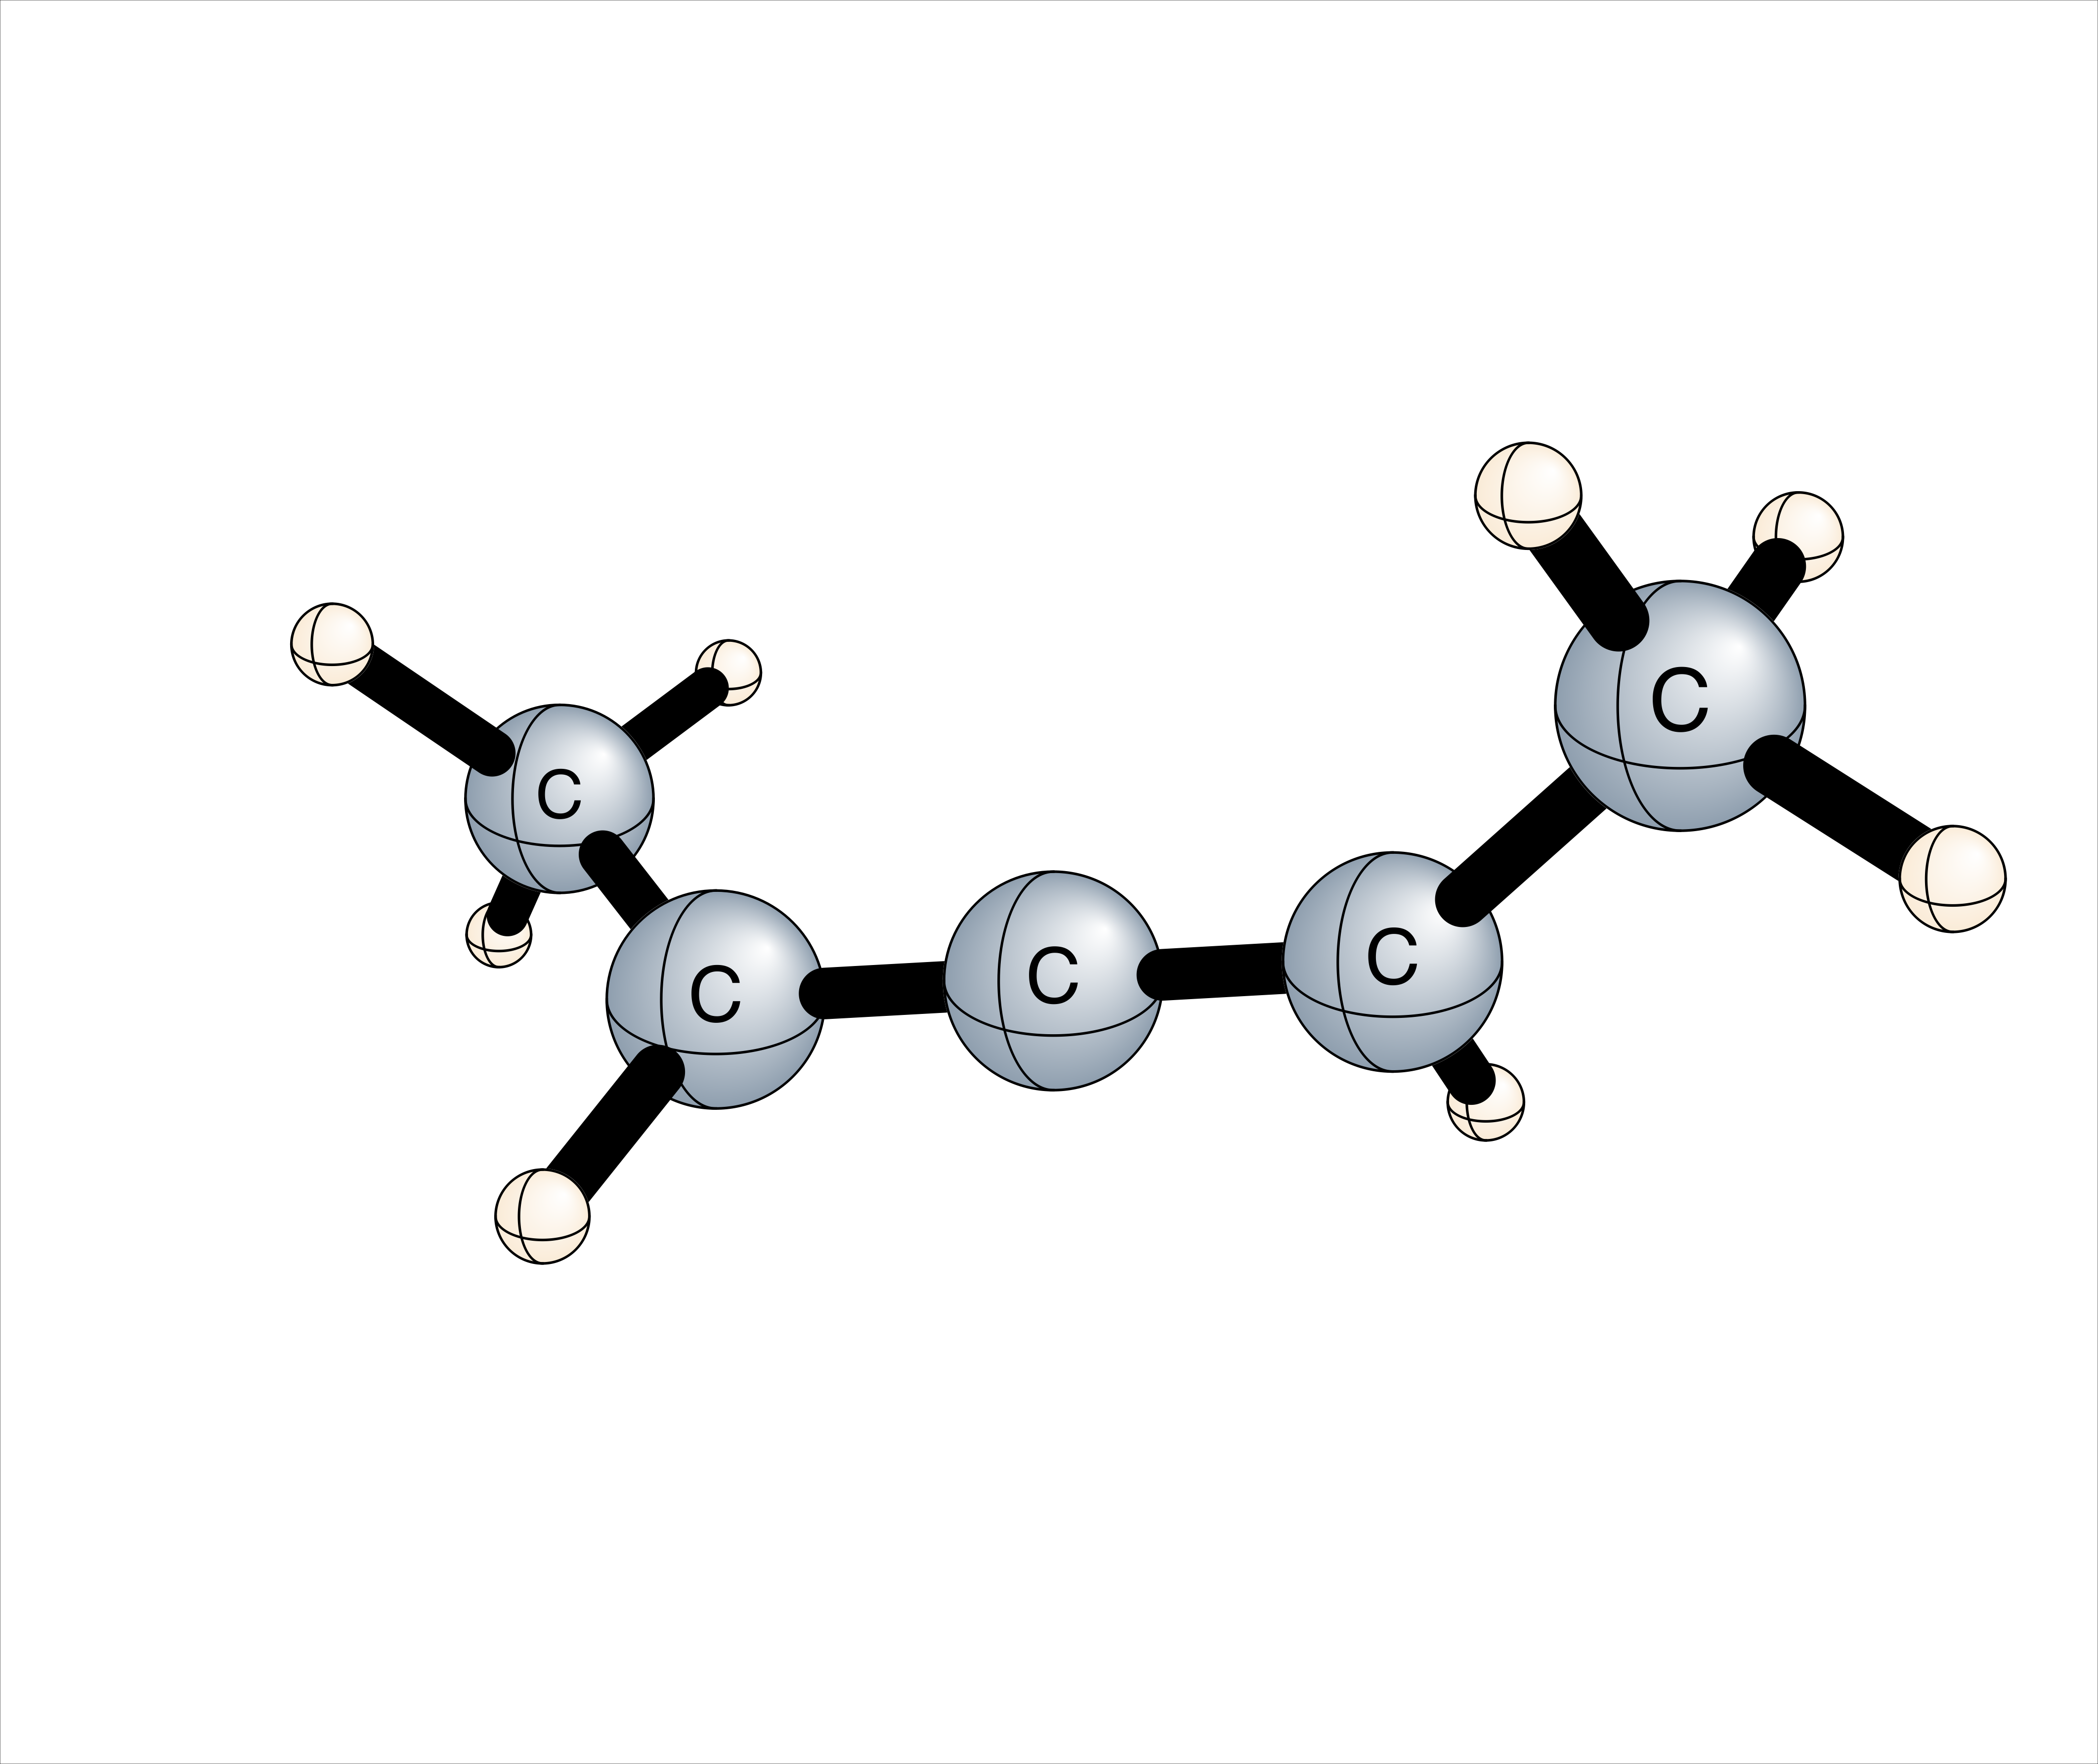
\includegraphics[scale=0.03]{pics/DMA.png}
%		\caption{\hskip 5em \textbf{(0)}}
%		%\label{fig:s1_3}
%	\end{subfigure}
%	\begin{subfigure}[h]{1.2in}
%		\centering
%		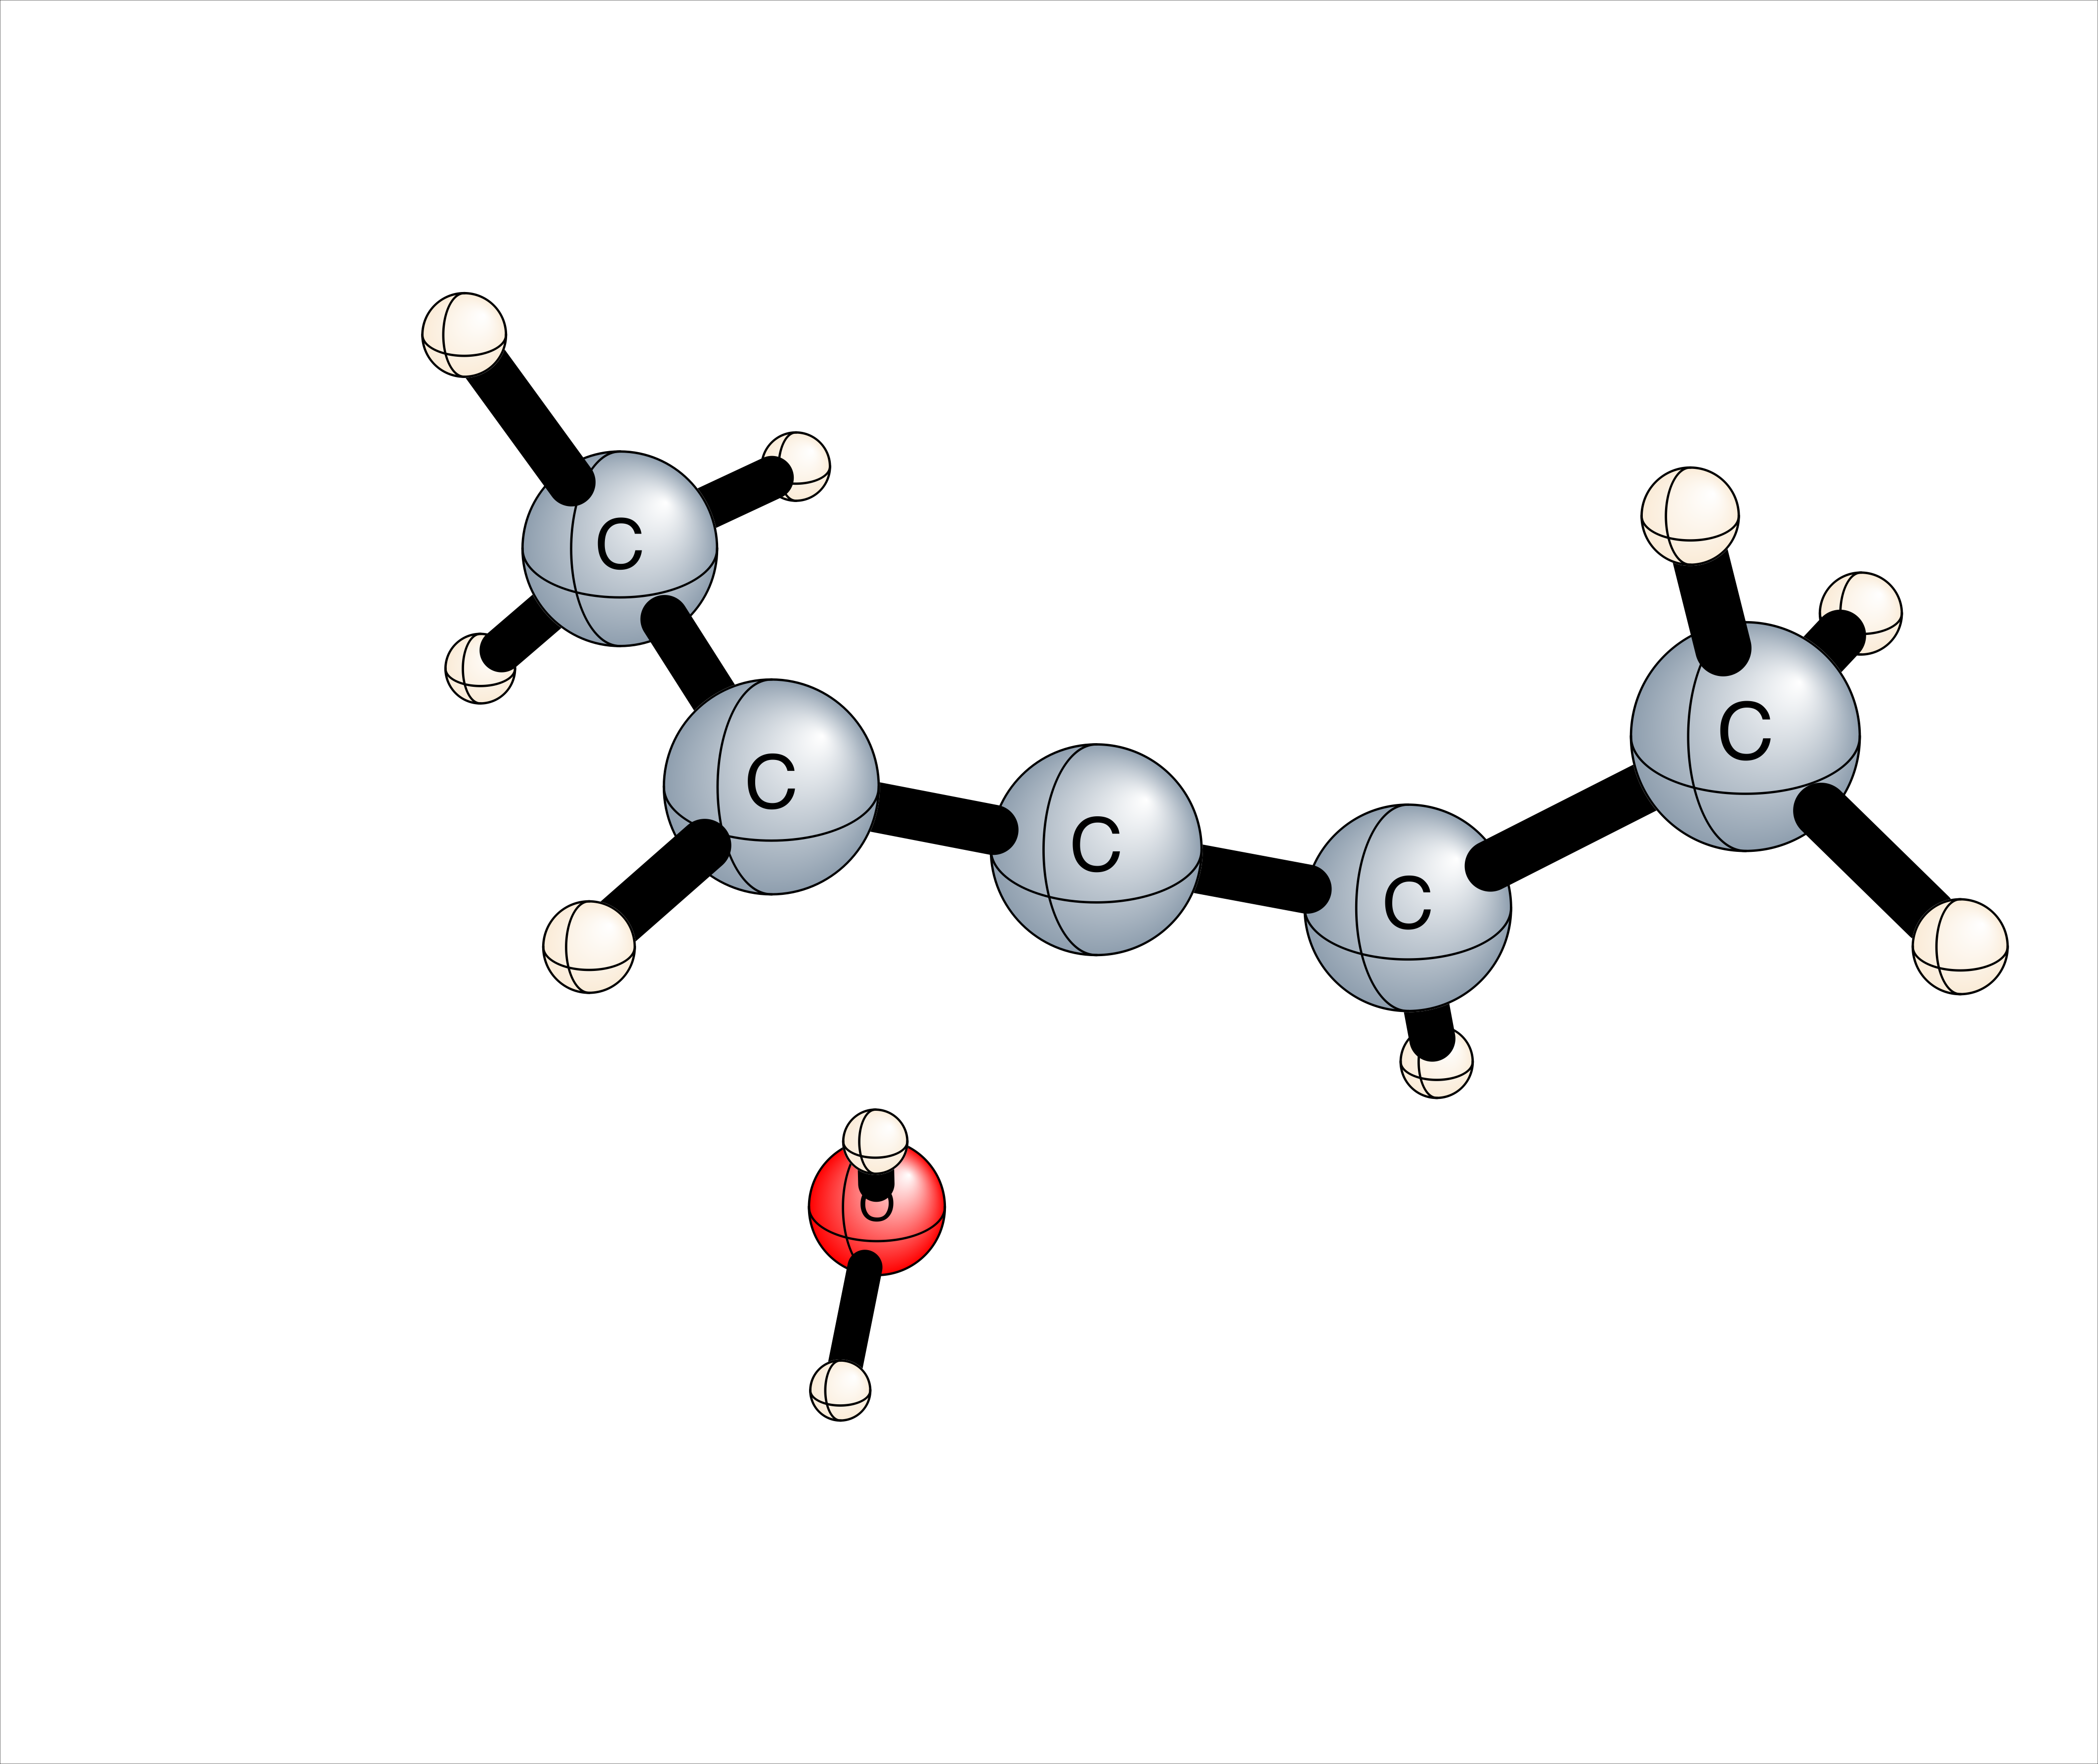
\includegraphics[scale=0.03]{pics/DMA_1w.png}
%		\caption{\hskip 4em \textbf{(1.3)}}
%		%\label{fig:s1_3}
%	\end{subfigure}
%	\begin{subfigure}[h]{1.2in}
%		\centering
%		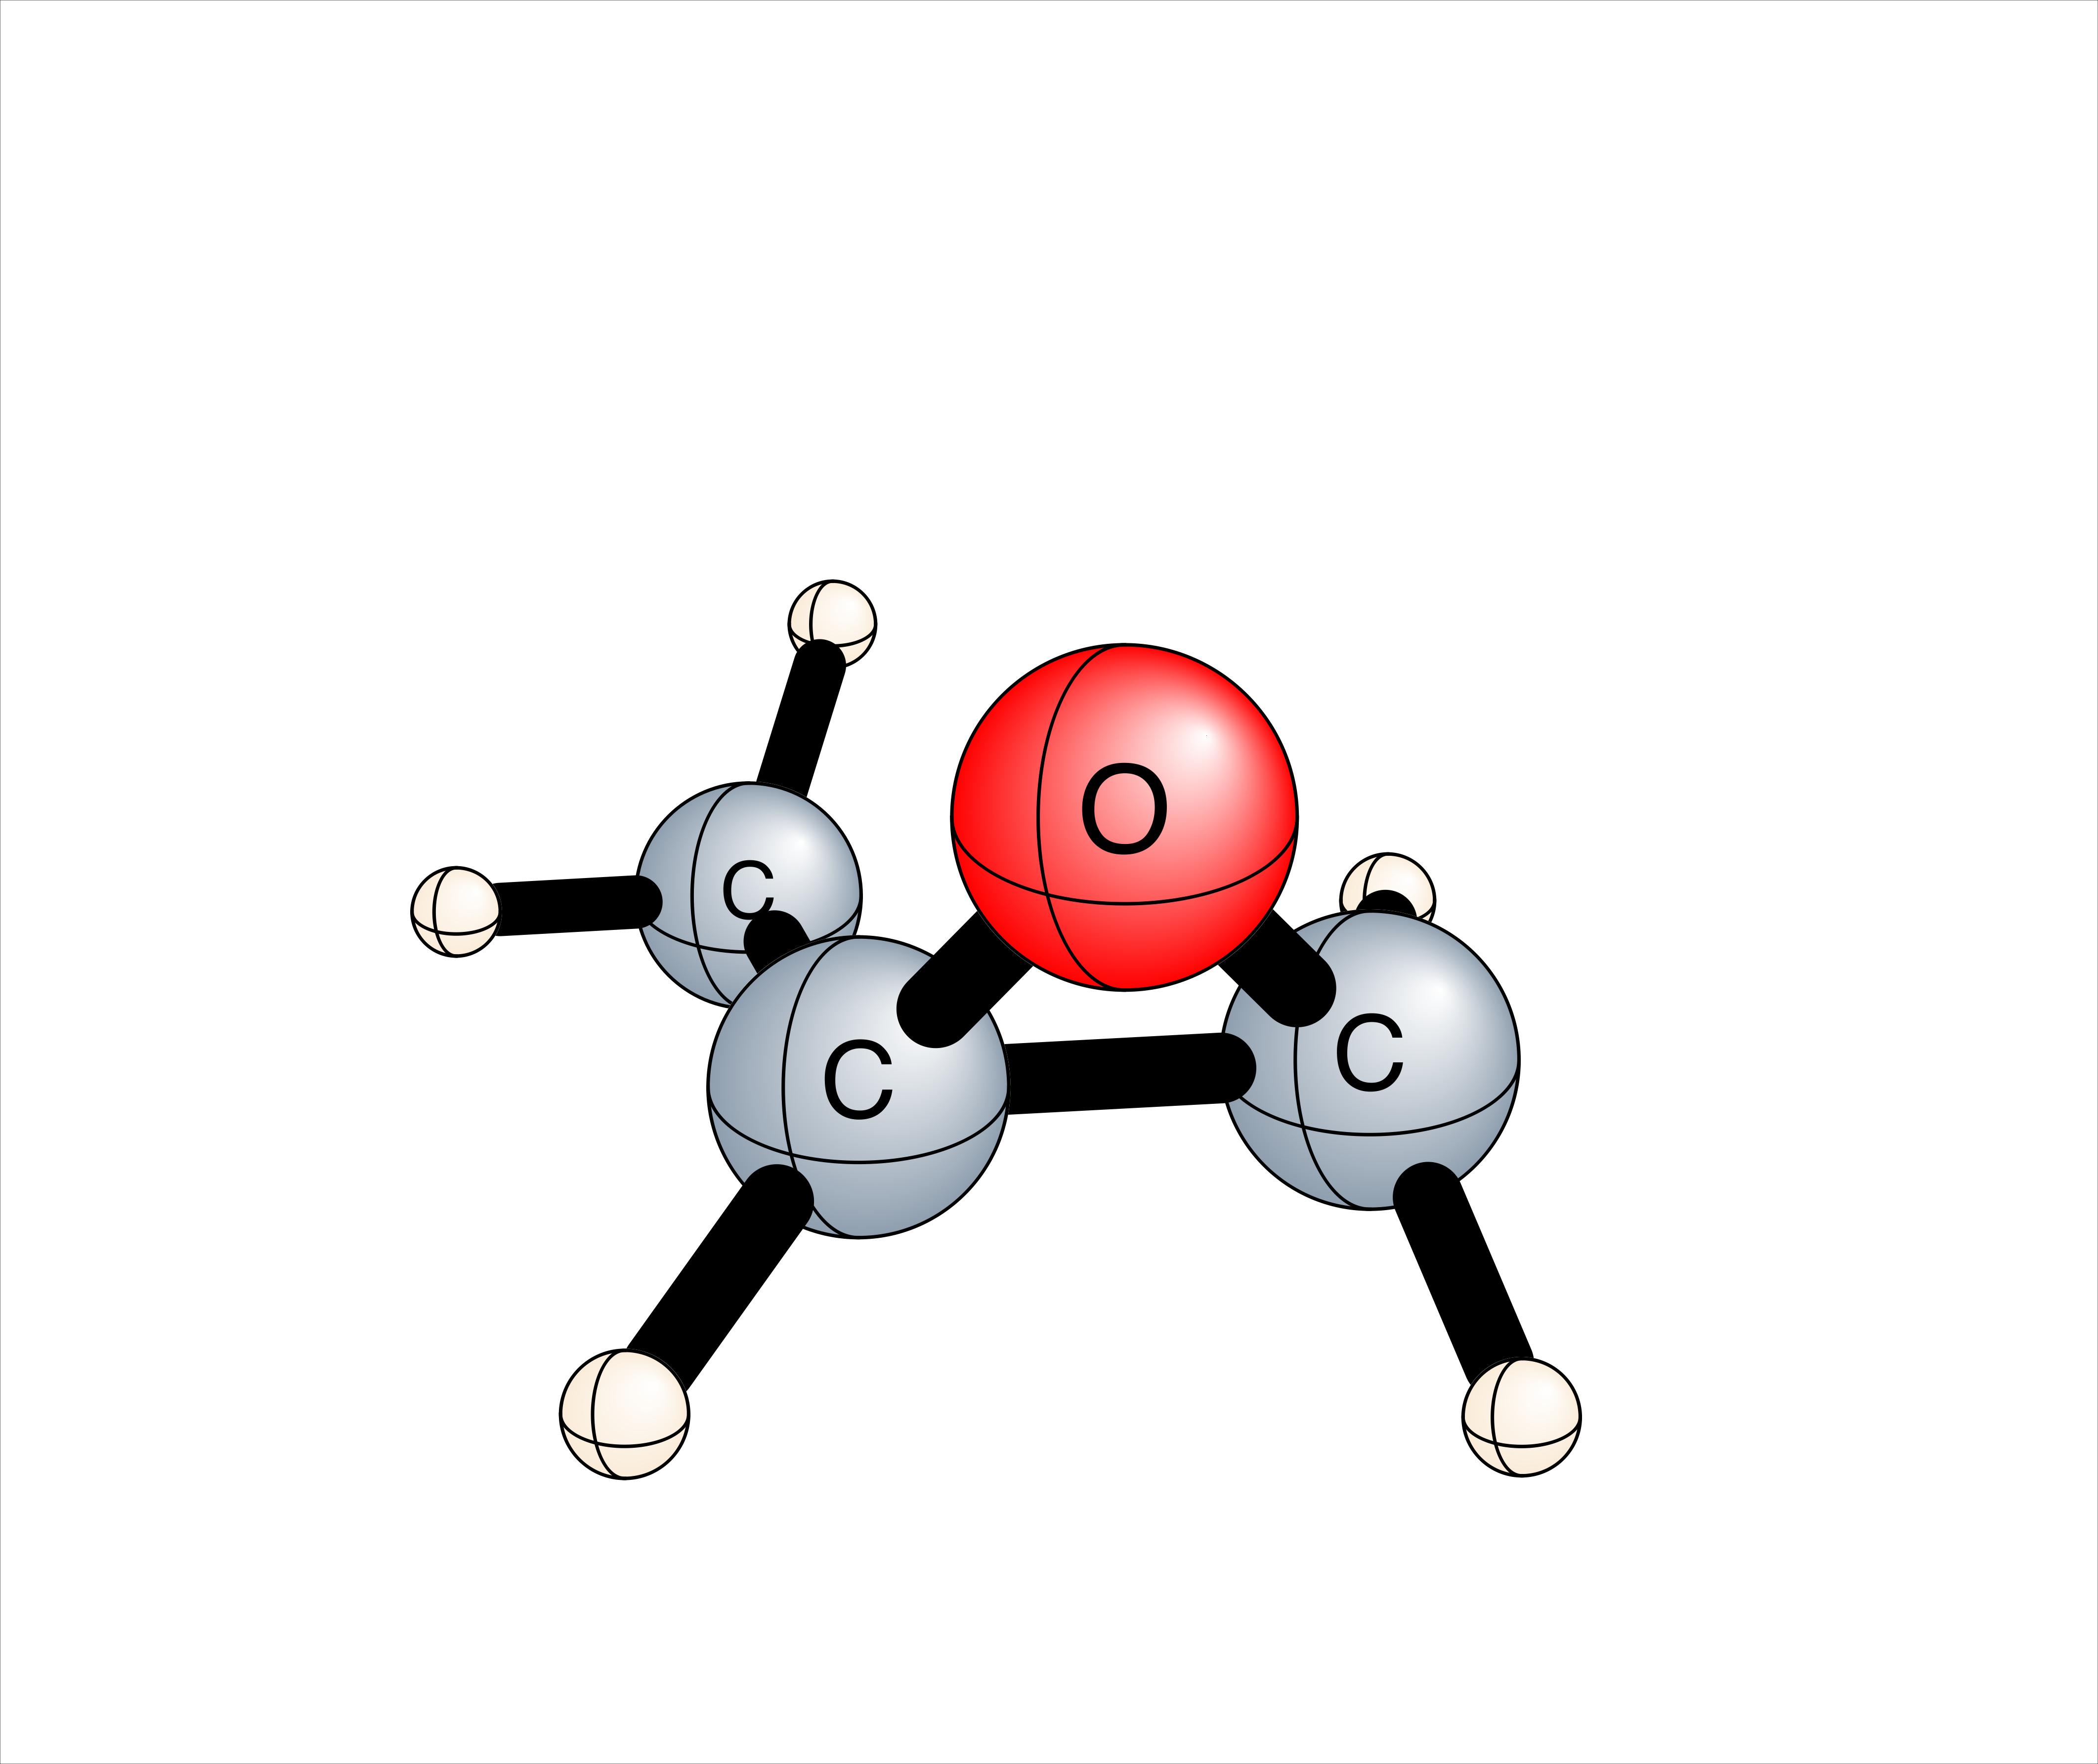
\includegraphics[scale=0.027]{pics/MOX.png}
%		\caption{\textbf{(2.3)}}
%		%\label{fig:s2_3}
%	\end{subfigure}
%	\begin{subfigure}[h]{1.2in}
%		\centering
%		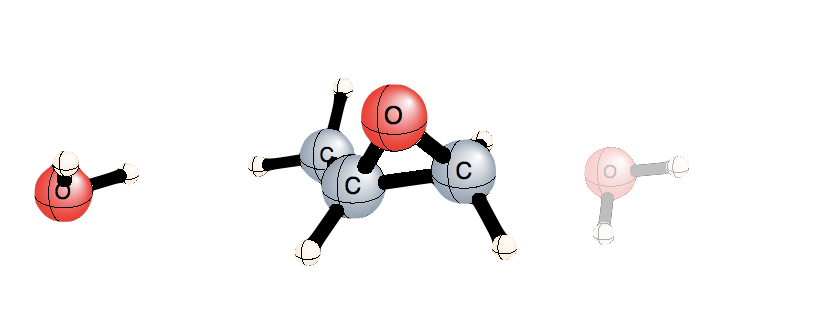
\includegraphics[scale=0.027]{pics/MOX_2w1g.png}
%		\caption{\textbf{(3.3)}}
%		%\label{fig:s3_3}
%	\end{subfigure}
% 	\begin{subfigure}[h]{1.2in}
%                \centering
%                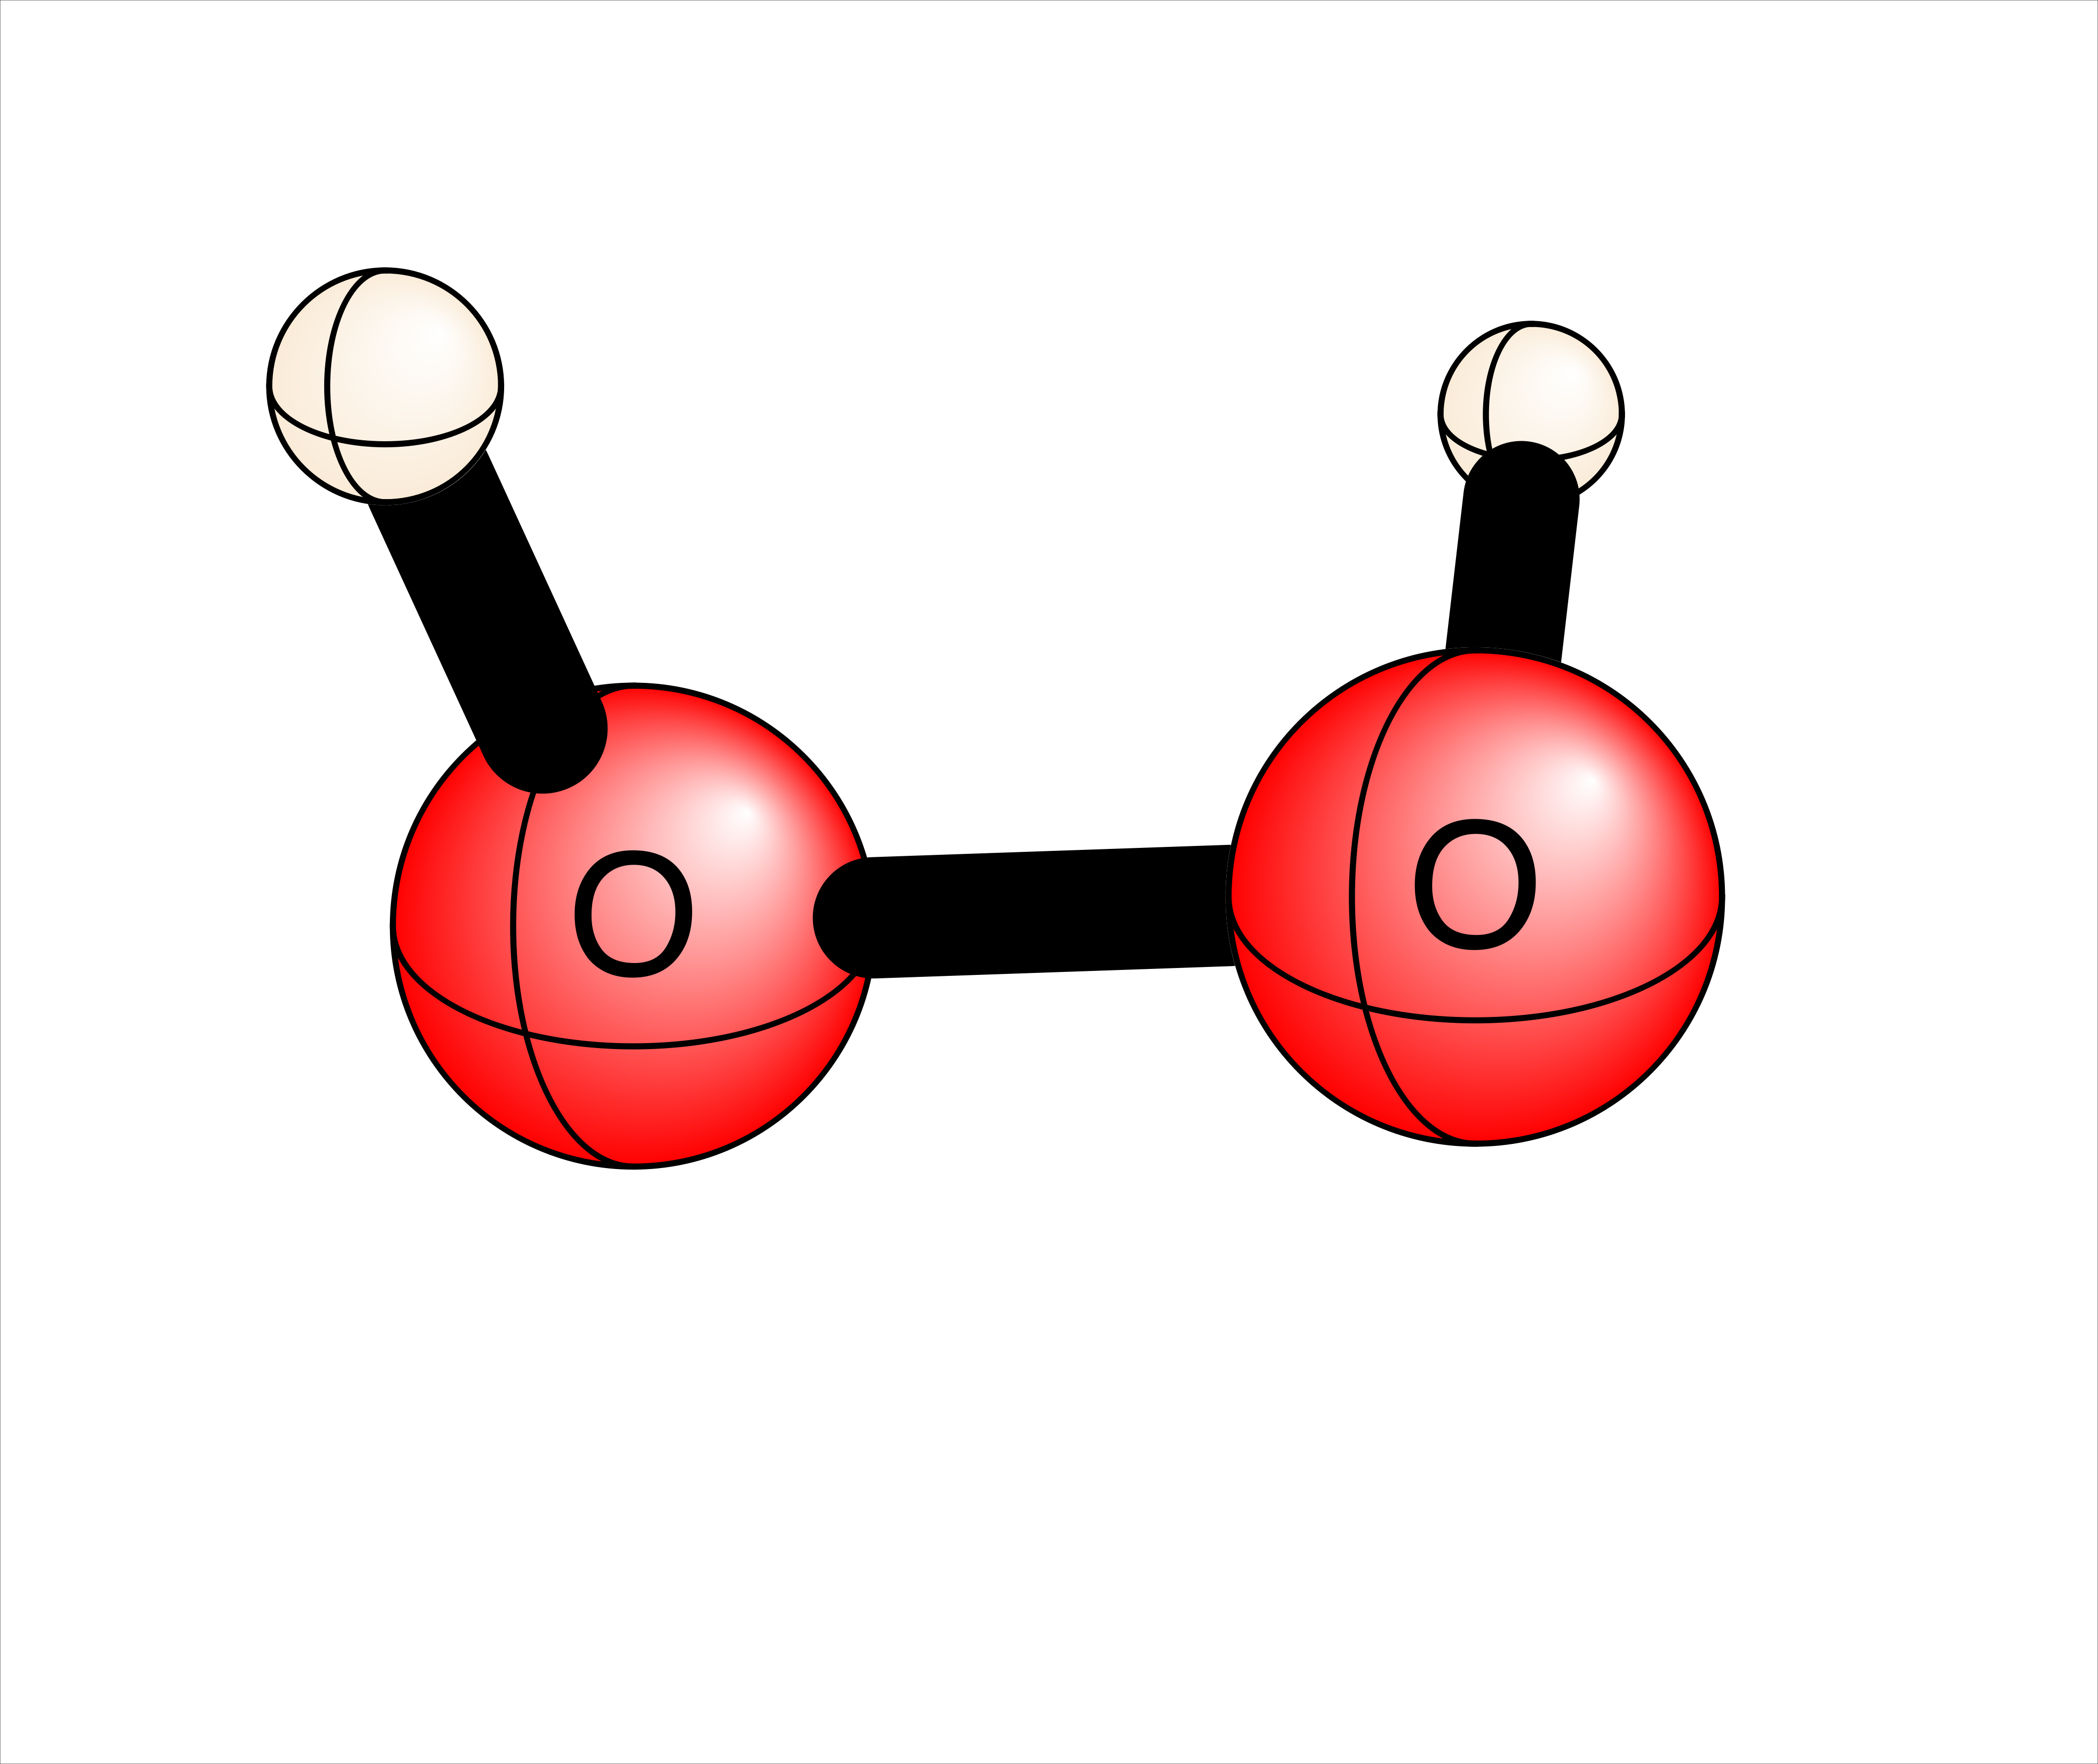
\includegraphics[scale=0.027]{pics/H2O2.png}
%                \caption{\textbf{(3.3)}}
%                %\label{fig:s3_3}
%        \end{subfigure}
%	\caption{Optimized structures of our test cases}
%	\label{fig:structs}
%\end{center}
%\end{figure}


\begin{figure}
\begin{subfigure}{.50\textwidth}
  \centering
  \includegraphics[width=1.1\linewidth]{pics/DMA.pdf}
  \caption{DMA}
  \label{fig:sfig1a}
\end{subfigure}
\hspace{0.1 in}
\begin{subfigure}{.50\textwidth}
  \centering
  \includegraphics[width=1.1\linewidth]{pics/MOX.pdf}
  \caption{MOX}
  \label{fig:sfig1b}
\end{subfigure}
\begin{subfigure}{.50\textwidth}
  \centering
  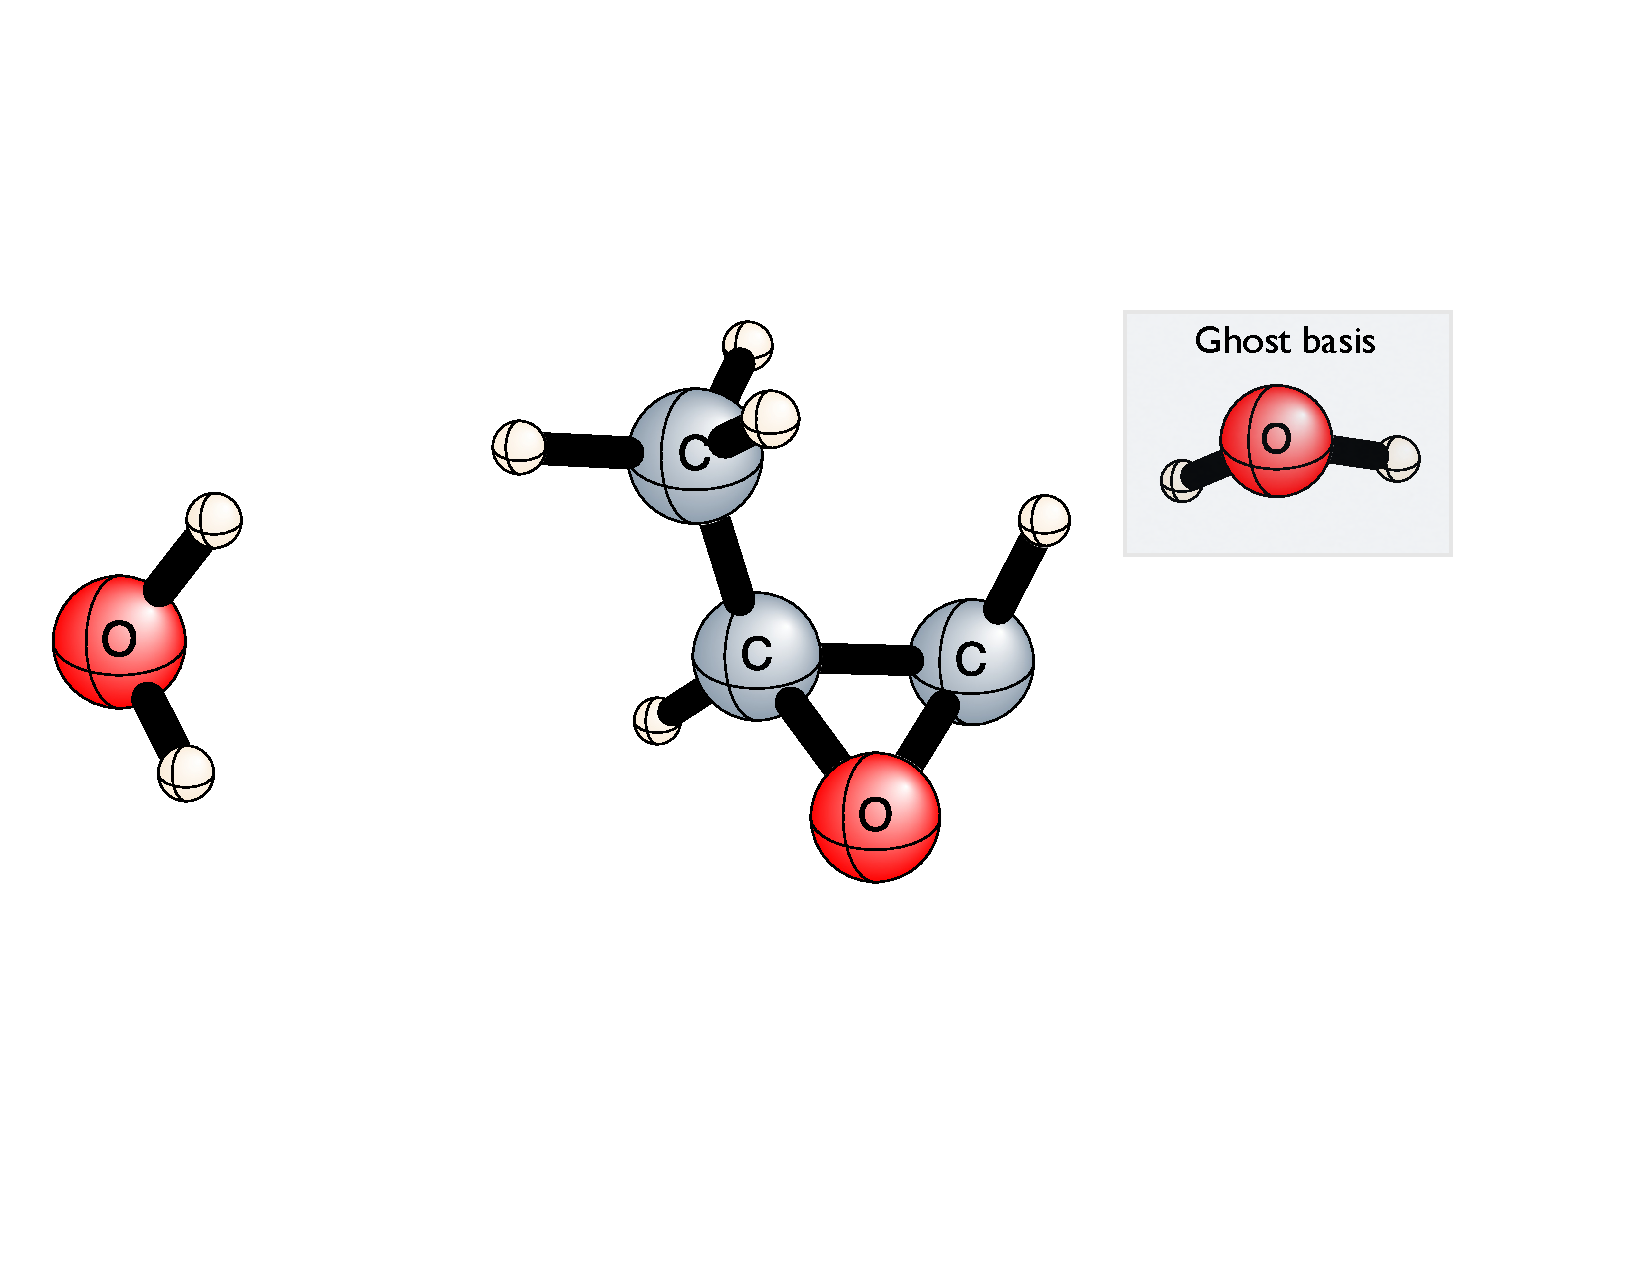
\includegraphics[width=1.1\linewidth]{pics/MOX_2w1g.pdf}
  \caption{MOX(2w1g)}
  \label{fig:sfig1c}
\end{subfigure}
\hspace{0.1 in}
\begin{subfigure}{.50\textwidth}
  \centering
  \includegraphics[width=1.1\linewidth]{pics/DMA_1w.pdf}
  \caption{DMA(1w)}
  \label{fig:sfig1d}
\end{subfigure}
\caption{Optimized geometries of test cases.}
\label{fig:fig1}
\end{figure}
